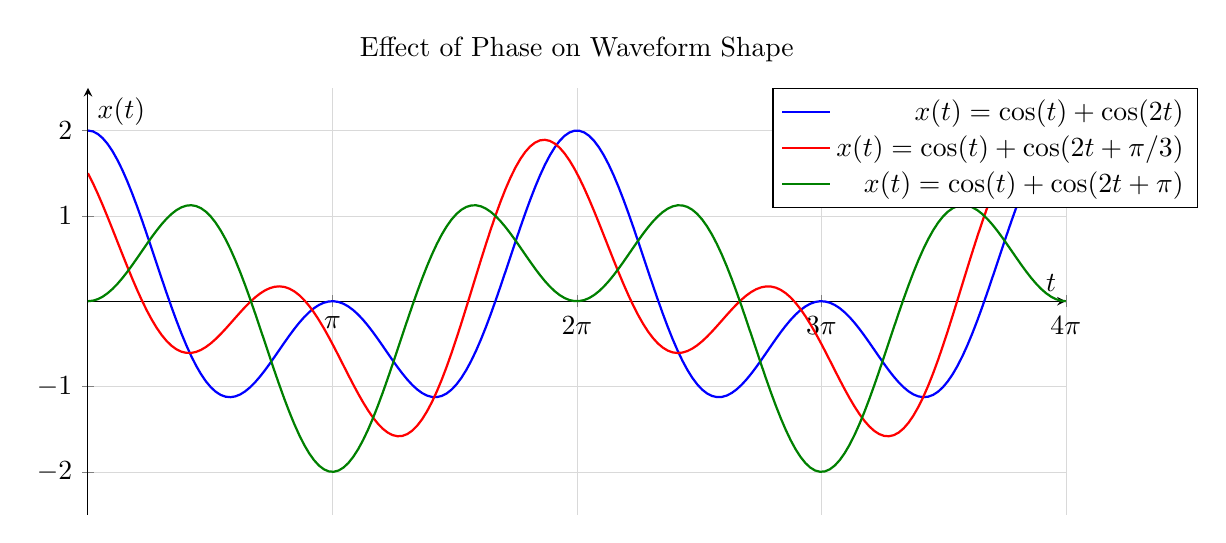
\begin{tikzpicture}
	\begin{axis}[
		width=14cm,
		height=7cm,
		title={Effect of Phase on Waveform Shape},
		xlabel={$t$},
		ylabel={$x(t)$},
		axis lines=middle,
		xmin=0, xmax=4*pi,
		ymin=-2.5, ymax=2.5,
		xtick={0, 3.14159, 6.28318, 9.42477, 12.56637},
		xticklabels={$0$,$\pi$,$2\pi$,$3\pi$,$4\pi$},
		ytick={-2,-1,1,2},
		grid=major,
		grid style={line width=.1pt, draw=gray!30},
		legend style={
			at={(0.7, 1)}, % 3% from left, 97% from bottom
			anchor=north west,   % Anchor the top-left corner of the legend
			legend cell align={right}
		},
		no marks,
		]
		% Case 1: phi = 0
		\addplot[blue, thick, domain=0:4*pi, samples=200] {cos(deg(x)) + cos(deg(2*x))};
		\addlegendentry{$x(t) = \cos(t) + \cos(2t)$};
		
		% Case 2: phi = pi/3
		\addplot[red, thick, domain=0:4*pi, samples=200] {cos(deg(x)) + cos(deg(2*x) + 60)};
		\addlegendentry{$x(t) = \cos(t) + \cos(2t + \pi/3)$};
		
		% Case 3: phi = pi
		\addplot[green!50!black, thick, domain=0:4*pi, samples=200] {cos(deg(x)) + cos(deg(2*x) + 180)};
		\addlegendentry{$x(t) = \cos(t) + \cos(2t + \pi)$};
	\end{axis}
\end{tikzpicture}

\begin{tikzpicture}
	% Define a style for the impulse plot
	\pgfplotsset{
		impulse/.style={
			ycomb, 
			blue, 
			thick, 
			mark=*, 
			mark size=2pt, 
			mark options={fill=blue}
		}
	}
	
	\begin{axis}[
		width=14cm,
		height=7cm,
		title={Magnitude Spectrum (Unaffected by Phase)},
		xlabel={$\omega$},
		ylabel={$|X(j\omega)|$},
		axis lines=middle,
		xmin=-3.5, xmax=3.5,
		ymin=0, ymax=4,
		xtick={-2,-1,1,2},
		ytick={3.14159},
		yticklabels={$\pi$},
		grid=major,
		grid style={line width=.1pt, draw=gray!30},
		]
		% Draw impulses at w = +/-1 and w = +/-2, all with height pi
		% The node near coords places the label 'π' above each impulse.
		\addplot[
		impulse,
		nodes near coords={$\pi$},
		every node near coord/.style={anchor=south, font=\small}
		] 
		coordinates {(-2,pi) (-1,pi) (1,pi) (2,pi)};
	\end{axis}
\end{tikzpicture}








